\documentclass{standalone}
\usepackage{tikz}
\usetikzlibrary{backgrounds}
\usetikzlibrary{plotmarks}
\usepackage{xcolor}
%
\definecolor{capmarvel}{HTML}{FED114}
\definecolor{capmarvelb}{HTML}{89230D}
\definecolor{caroldanversa}{HTML}{FB0E14}
\definecolor{caroldanversb}{HTML}{1D9B8F}
%
\usepackage{mathptmx}
%
\title{Captain Marvel}
\begin{document}
	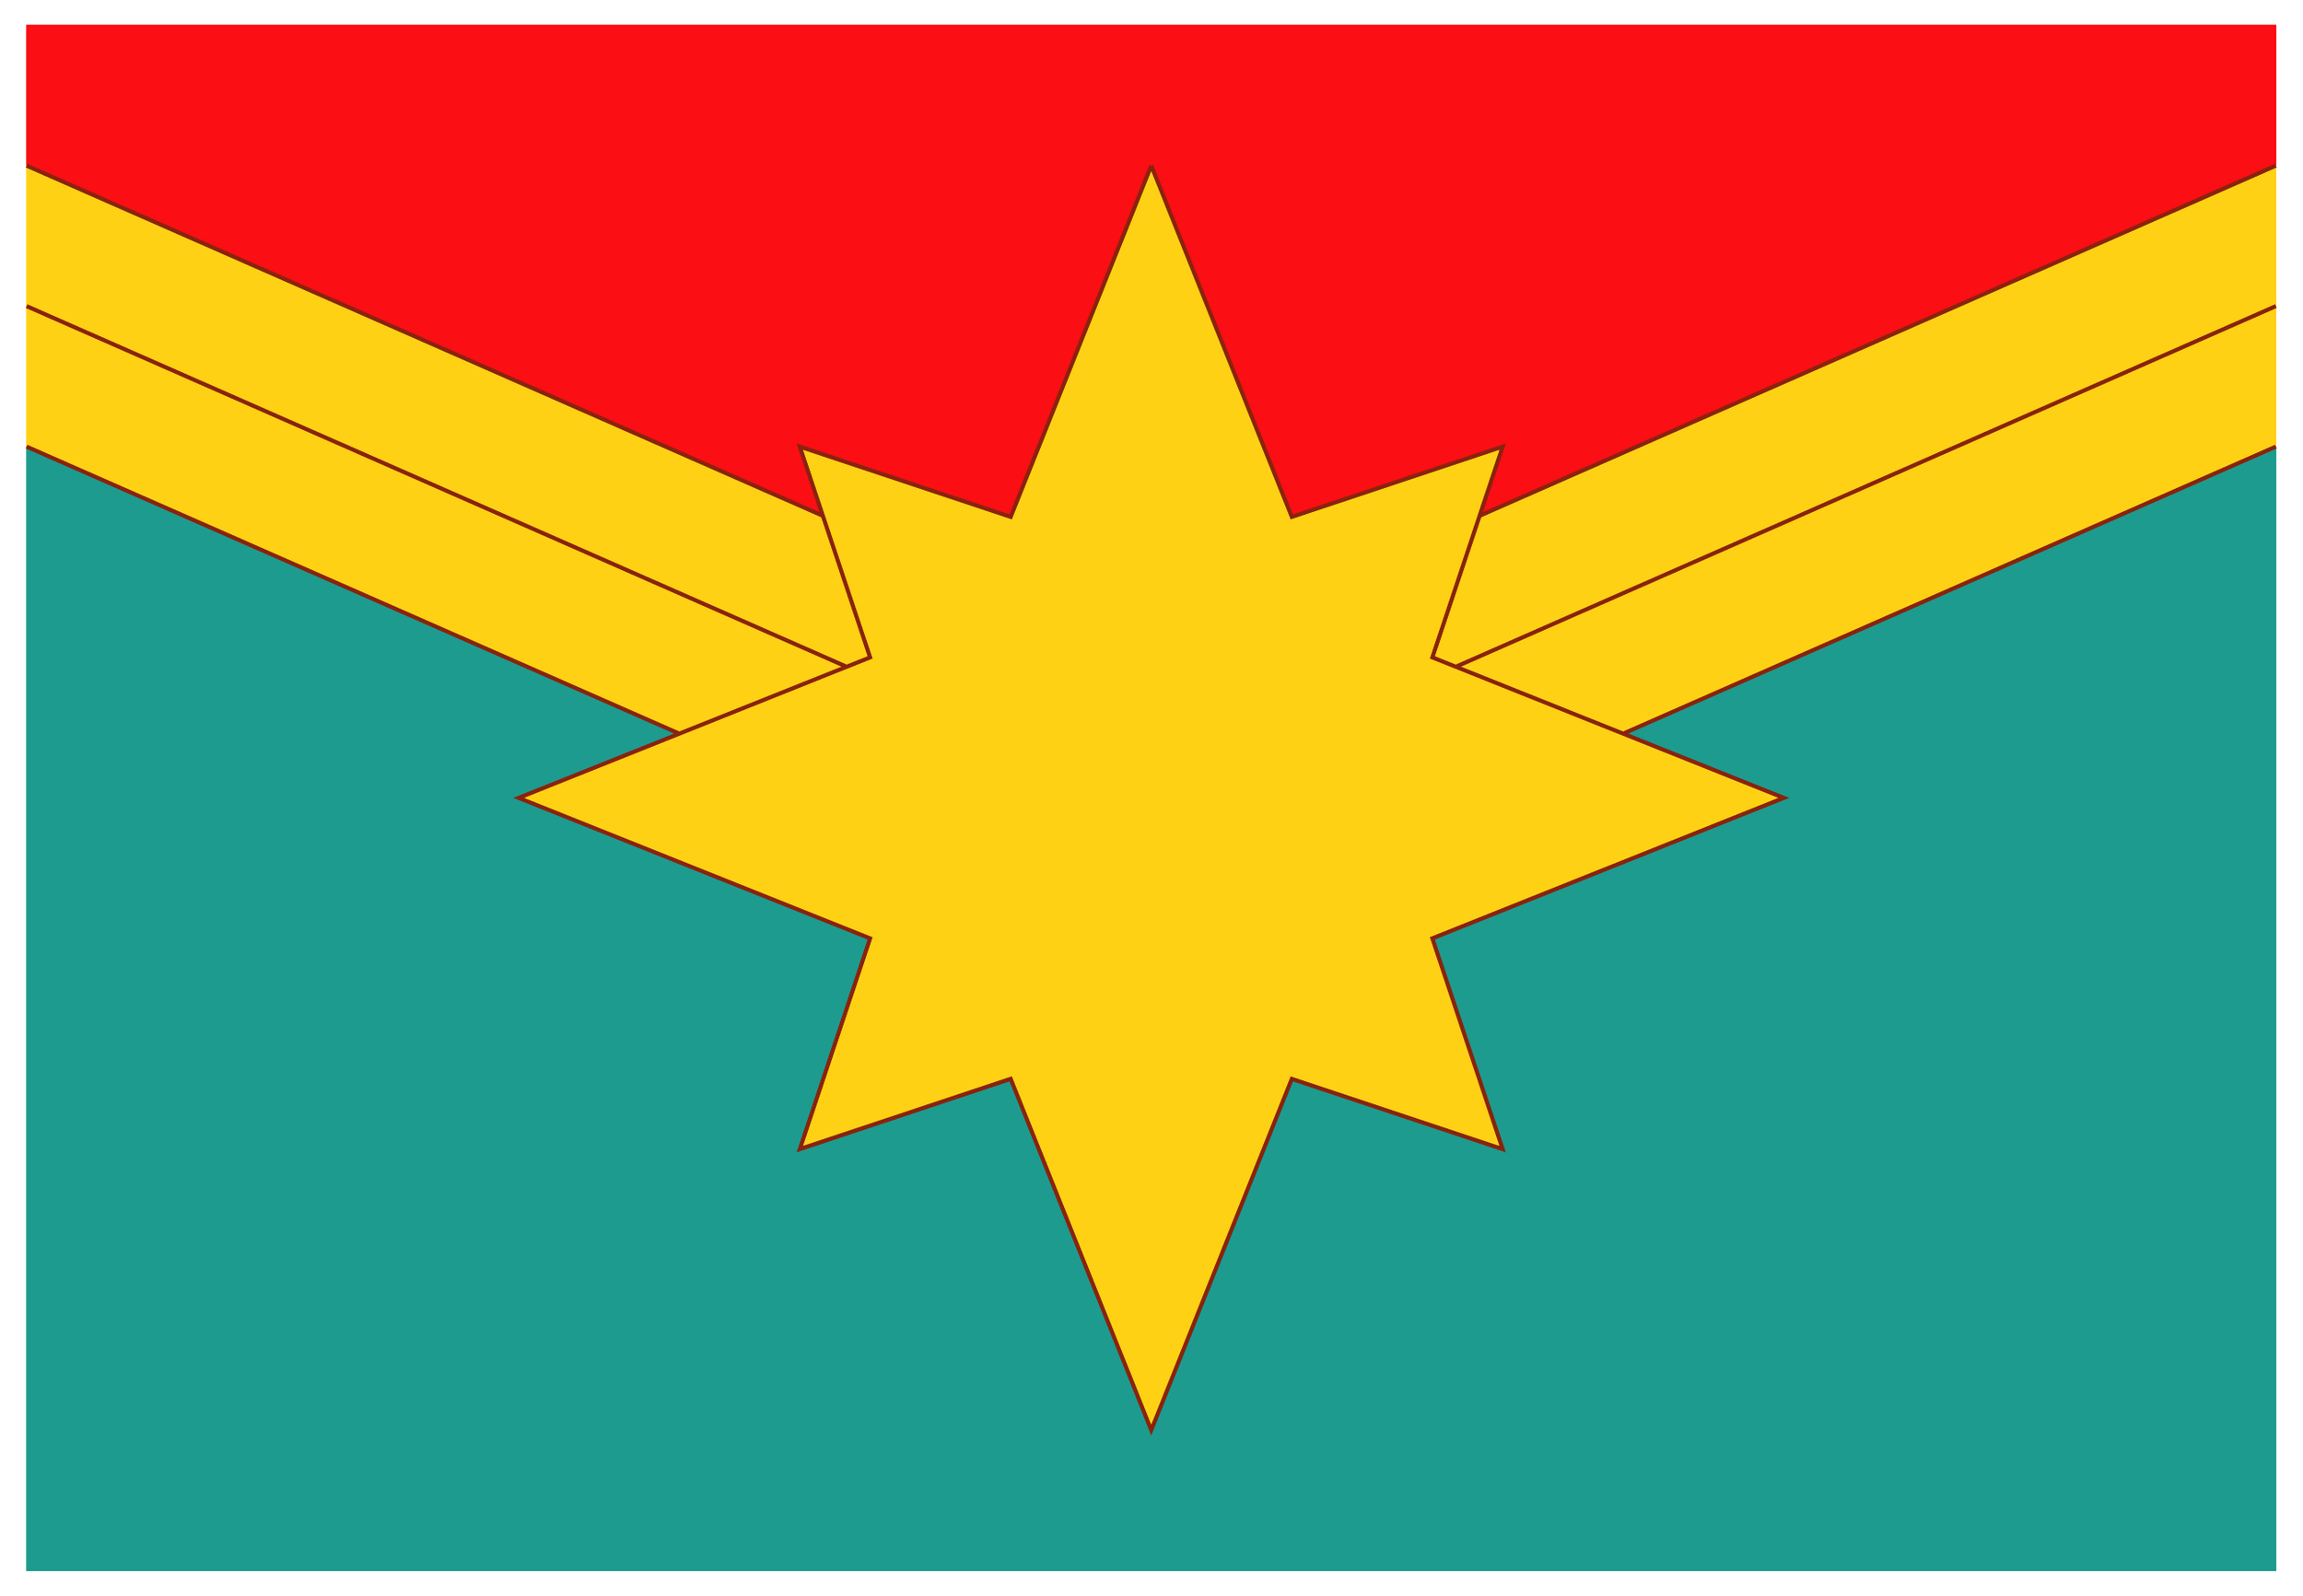
\begin{tikzpicture}
		\draw[color=caroldanversa,fill=caroldanversa] (16,9) -- (16,11) -- (-16,11) -- (-16,9) -- (0,1.8) -- (16,9);
		\draw[color=caroldanversb,fill=caroldanversb] (16,5) -- (16,-11) -- (-16,-11) -- (-16,5) -- (0,-1.8) -- (16,5);
		%
		\draw[color=capmarvel,fill=capmarvel] (3.5,3.5) -- (16,9) -- (16,5) -- (3.5,-0.5) -- (3.5,3.5);
		\draw[ultra thick, color=capmarvelb] (3.5,3.5) -- (16,9);
		\draw[ultra thick, color=capmarvelb] (3.5,1.5) -- (16,7);
		\draw[ultra thick, color=capmarvelb] (3.5,-0.5) -- (16,5);
		%
		\draw[color=capmarvel,fill=capmarvel] (-3.5,3.5) -- (-16,9) -- (-16,5) -- (-3.5,-0.5) -- (-3.5,3.5);
		\draw[ultra thick, color=capmarvelb] (-3.5,3.5) -- (-16,9);
		\draw[ultra thick, color=capmarvelb] (-3.5,1.5) -- (-16,7);
		\draw[ultra thick, color=capmarvelb] (-3.5,-0.5) -- (-16,5);
		%
		\draw[ultra thick,color=capmarvelb,fill=capmarvel] (0,9) -- (2,4) -- (5,5) -- (4,2) -- (9,0) -- (4,-2) -- (5,-5) -- (2,-4) -- (0,-9) -- (-2,-4) -- (-5,-5) -- (-4,-2) -- (-9,0) -- (-4,2) -- (-5,5) -- (-2,4) -- (0,9);
	\end{tikzpicture}
%
\end{document}